\documentclass[tikz,border=10pt]{standalone}
\usetikzlibrary{positioning, arrows.meta, calc, patterns, babel, fit, backgrounds}
\usepackage[utf8]{inputenc}
\usepackage[T1]{fontenc}
\usepackage{lmodern}
\usepackage[english]{babel}
\usepackage{amsmath, amssymb, bm}

\begin{document}
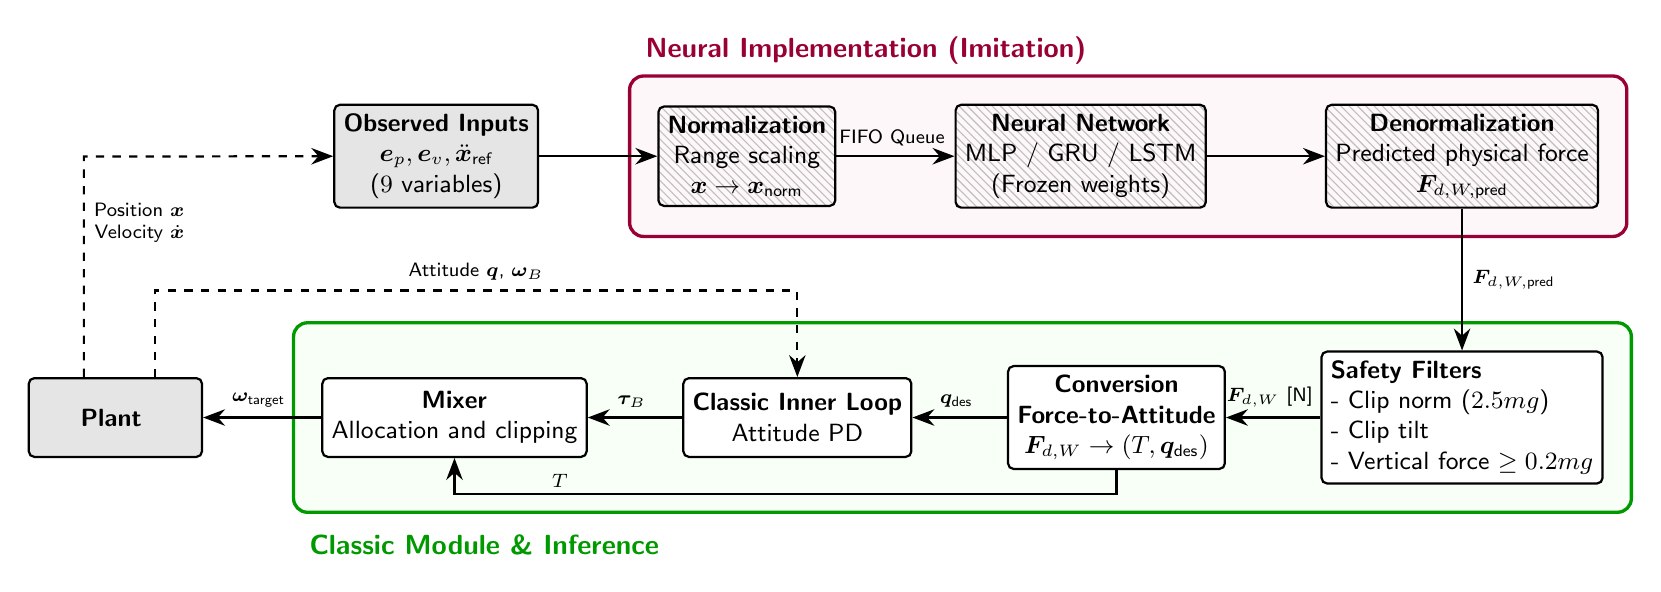
\begin{tikzpicture}[
  node distance=0.8cm and 1.0cm,
  align=center,
  font=\sffamily\small,
  % Estilos de bloques
  box/.style={draw, rectangle, rounded corners=2pt, minimum width=2.2cm, minimum height=1.0cm, thick, fill=white},
  groupbox/.style={draw, rectangle, rounded corners=5pt, line width=1.2pt, inner sep=10pt},
  neuralbox/.style={box, fill=black!5, pattern=north west lines, pattern color=black!25},
  % Estilos de flechas
  line/.style={draw, -{Stealth[scale=1.2]}, thick},
  dashline/.style={draw, -{Stealth[scale=1.2]}, thick, dashed}
]

  % ==========================================
  % UPPER ROW: NEURAL POLICY (LEARNED - PATTERNED)
  % ==========================================
  \node[box, fill=black!10] (entradas) at (-2, 3.2) {
    \textbf{Observed Inputs}\\
    $\bm{e}_p, \bm{e}_v, \ddot{\bm{x}}_{\text{ref}}$\\
    ($9$ variables)
  };
  
  \node[neuralbox, right= 1.5cm of entradas] (normalizador) {
    \textbf{Normalization}\\
    Range scaling\\
    $\bm{x} \to \bm{x}_{\text{norm}}$
  };

  \node[neuralbox, right=1.5cm of normalizador] (red) {
    \textbf{Neural Network}\\
    MLP / GRU / LSTM\\
    (Frozen weights)
  };

  \node[neuralbox, right= 1.5cm of red] (desnormalizador) {
    \textbf{Denormalization}\\
    Predicted physical force\\
    $\bm{F}_{d,W,\text{pred}}$
  };

  \draw[line] (entradas) -- (normalizador);
  \draw[line] (normalizador) -- node[above, font=\sffamily\scriptsize] {FIFO Queue} (red);
  \draw[line] (red) -- (desnormalizador);

  % ==========================================
  % LOWER ROW: INNER LOOP AND CLASSICAL PROTECTIONS
  % ==========================================
  \node[box, below=1.8cm of desnormalizador, fill=white, align=left] (clipping) {
    \textbf{Safety Filters}\\
    - Clip norm ($2.5mg$)\\
    - Clip tilt\\
    - Vertical force $\ge 0.2mg$
  };
  \draw[line] (desnormalizador) -- node[right, font=\sffamily\scriptsize] {$\bm{F}_{d,W,\text{pred}}$} (clipping);

  \node[box, left=1.2cm of clipping, fill=white] (conversion) {
    \textbf{Conversion}\\
    \textbf{Force-to-Attitude}\\
    $\bm{F}_{d,W} \to (T, \bm{q}_{\text{des}})$
  };
  \draw[line] (clipping) -- node[above, font=\sffamily\scriptsize] {$\bm{F}_{d,W}$ [N]} (conversion);

  \node[box, left=1.2cm of conversion, fill=white] (lazo_interno) {
    \textbf{Classic Inner Loop}\\
    Attitude PD
  };
  \draw[line] (conversion) -- node[above, font=\sffamily\scriptsize] {$\bm{q}_{\text{des}}$} (lazo_interno);

  \node[box, left=1.2cm of lazo_interno, fill=white] (mixer) {
    \textbf{Mixer}\\
    Allocation and clipping
  };
  \draw[line] (lazo_interno) -- node[above, font=\sffamily\scriptsize] {$\bm{\tau}_B$} (mixer);
  \draw[line] (conversion.south) |- ++(-1.5, -0.3) -| node[pos=0.4, yshift=-0.05cm, above, font=\sffamily\scriptsize] {$T$} (mixer.south);

  % ==========================================
  % CONTEXT GROUPS
  % ==========================================
  \begin{scope}[on background layer]
    % Contenedor Bloque Neuronal Aprendido
    \node[groupbox, draw=purple!80!black, fill=purple!3, fit=(normalizador) (red) (desnormalizador)] (neural_group) {};
    
    % Contenedor Bloque Clásico
    \node[groupbox, draw=green!60!black, fill=green!3, fit=(clipping) (conversion) (lazo_interno) (mixer)] (classic_group) {};
  \end{scope}

  \node[anchor=south west, font=\sffamily\bfseries, color=purple!80!black] at ($(neural_group.north west) + (0.1,0)$) {Neural Implementation (Imitation)};
  \node[anchor=north west, font=\sffamily\bfseries, color=green!60!black] at ($(classic_group.south west) + (0.1,-0.15)$) {Classic Module \& Inference};

  % ==========================================
  % PLANT AND FEEDBACKS
  % ==========================================
  \node[box, left=1.5cm of mixer, fill=gray!20] (planta) {
    \textbf{Plant}
  };
  \draw[line] (mixer) -- node[above, font=\sffamily\scriptsize] {$\bm{\omega}_{\text{target}}$} (planta);

  % 1. Position feedback to inputs
  \draw[dashline] ([xshift=-0.4cm]planta.north) -- ++(0, 2.8) node[pos=0.7, right, align=right, font=\sffamily\scriptsize] {Position $\bm{x}$\\Velocity $\dot{\bm{x}}$} -- (entradas.west);

  % 2. Attitude feedback to classic inner loop
  \draw[dashline] ([xshift=0.5cm]planta.north) -- ++(0, 1.1) coordinate (fb_att) -| (lazo_interno.north);
  \node[above, font=\sffamily\scriptsize] at ($(fb_att)!0.5!(lazo_interno.north |- fb_att)$)
    {Attitude $\bm{q}$, $\bm{\omega}_B$};

\end{tikzpicture}
\end{document}
